\subsubsection{roBERTa}
RoBERTa is a bidirectional pretrained encoder based on BERT, but trained on a larger amount of data and with longer sequences. BERT itself is based on the encoder component of the Transformer architecture, which generates vector representations by considering both the past and future context of the sequence elements. The pretrained knowledge of the model can be reused for other tasks by simply adding a classification head and fine-tuning the pretrained weights to solve the new problem. In \cite{bonetti2021hate}, BERTweet was used — a model similar to RoBERTa but specifically trained on Twitter data — achieving an accuracy of 92.38.

\subsubsection{Methodology XGBoost}

The methodology used for the XGBoostClassifier began by loading the [CLS] token embeddings generated by RoBERTa, that is, the vector that summarizes the entire text sequence. After this, the data was split into 80\% for training and 20\% for testing. This split resulted in 38,152 examples available for training. Subsequently, a parameter grid was defined to conduct hyperparameter tuning. The search focused on the number of estimators, maximum tree depth, and minimum child weight. To find the best values, a grid search with 3-fold cross-validation was used.

In addition to this search, other hyperparameters were set manually. For example, 80\% of the data was used in each boosting round, and in each tree and node, a sample of features was selected such that its size was proportional to the square root of the total number of features, as recommended in \cite{Chen2016XGBoost}.

For training, 50\% of the dataset was used to perform the hyperparameter search, as doing it on the entire training set would have been computationally too expensive. Once the best hyperparameters were found, the model was trained on the full training set and then evaluated.

To evaluate the model, a classification report was generated that measured precision, recall, F1-score, and accuracy. Additionally, a confusion matrix was presented to more clearly observe the trend of the data toward true positives or misclassification.

\subsubsection{Methodology BI-LSTM}

For the model based on the BI-LSTM architecture, the full embeddings generated by the roBERTa model were used, and the architecture shown in Figure~\ref{fig:bilstm_architecture}, as recommended in \cite{zhang2018deep}, was implemented. This architecture was trained using the Adam optimizer for 200 epochs, storing the checkpoint that achieved the highest accuracy on the validation set. This validation set accounted for 15\% of the data, as did the test set, while the remaining 70\% was used for training. 

After training, the best checkpoint was restored and performance evaluation was carried out. The model was assessed using the same metrics as with the XGBoostClassifier: precision, recall, F1-score, accuracy, and the confusion matrix.

\begin{figure}[htbp]
  \centering
  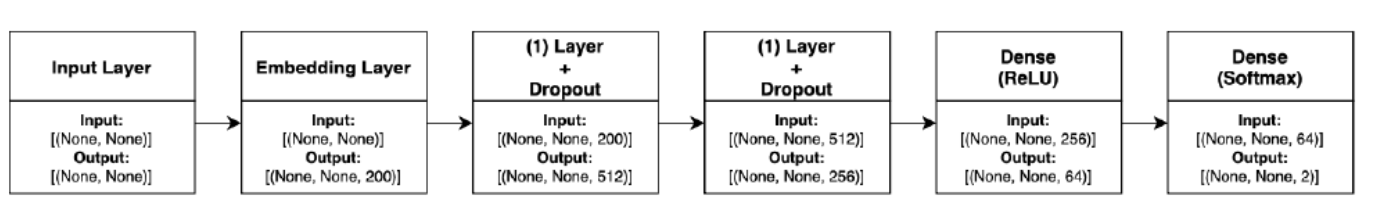
\includegraphics[width=0.45\textwidth]{images/bilstm_architecture.png}
  \caption{BI-LSTM architecture used in the model.}
  \label{fig:bilstm_architecture}
\end{figure}